\documentclass[assd_tp2_main.tex]{subfiles}

\begin{document}

\section{Efectos de audio}

\subsection{Reverbebrador}

\subsubsection{Implementación de eco simple}

Se implementó un eco simple utilizando el sistema

\begin{equation}
	y(n)=x(n)+gx(n-M)
\end{equation}

Se muestran a continuación los resultados con una señal de prueba

\begin{figure}[H]	
	\centering
	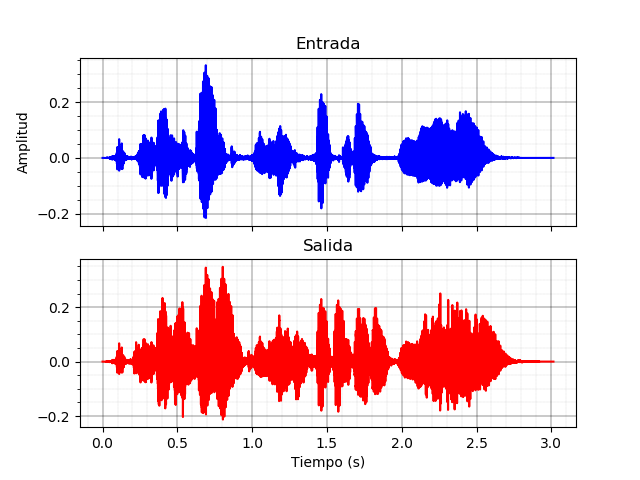
\includegraphics[scale=1]{graficos/EJ8/eco_simple.png}
	\caption{Resultados con $M=5000$, $g=0.999$ }
	\label{fig:bloqueElemental}
\end{figure}

Se puede observar de los resultados intuitivamente como la señal de salida contiene repeticiones de la señal de entrada, y al escuchar el audio se pudo notar dicho efecto de eco. Fue necesario colocar un retraso muy grande ($M=5000$) y una ganancia muy alta ($g=0.999$) para que el efecto fuera notorio

\subsubsection{Implementación de reverberación plana}
Se implementó una reverberación plana utilizando una ecuación de diferencias con feedback. 
\begin{equation}
	y(n)=x(n)+gy(n-M)
\end{equation}
Se muestran a continuación los resultados con una señal de prueba
\begin{figure}[H]	
	\centering
	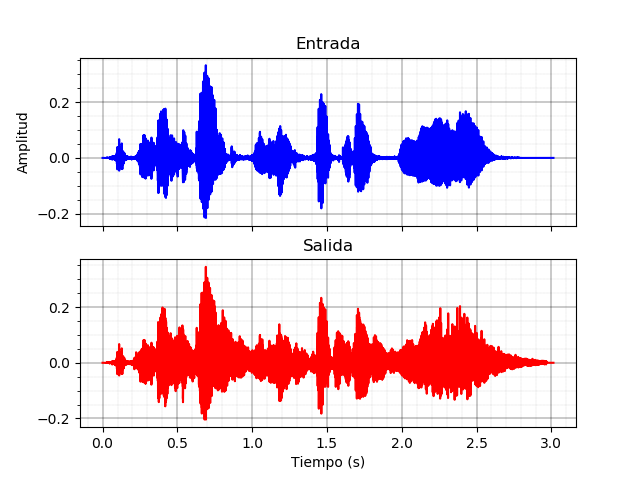
\includegraphics[scale=1]{graficos/EJ8/eco_plano.png}
	\caption{Resultados reverberación plana con $M=500$, $g=0.5$ }
	\label{fig:bloqueElemental}
\end{figure}
Se necesitó disminuir fuertemente el valor de $g$ para evitar que la salida saturara. Al tener realimentación (es decir, ser IIR) el sistema puede perder la estabilidad con facilidad

\subsubsection{Implementación de reverberación pasa bajos}

Se le agrego un filtro pasabajo a la realimentación del sistema anterior. Se optó por un sencillo pasabajos similar al utilizado en el modelo Karplus Strong, de la forma $y(n)=\frac{x(n)+x(n-1)}{2}$
El sistema por lo tanto quedo descrito como
\begin{equation}
y(n)=x(n)+\frac{1}{2}g(y(n-M)+y(n-M-1))
\end{equation}
\begin{figure}[H]	
	\centering
	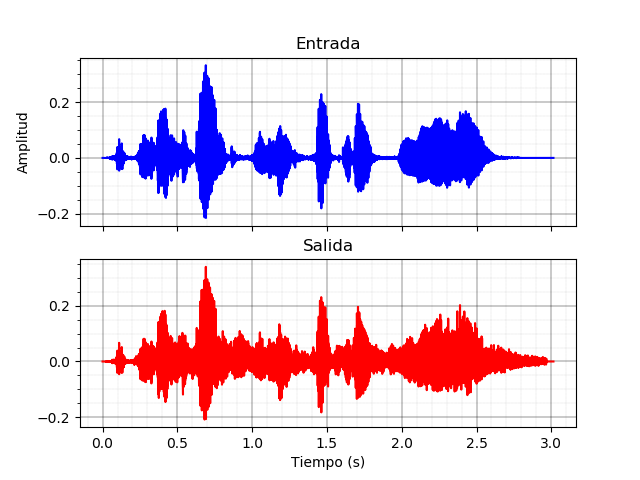
\includegraphics[scale=1]{graficos/EJ8/eco_pb.png}
	\caption{Resultados reververación con pasabajos $M=500$, $g=0.5$ }
	\label{fig:bloqueElemental}
\end{figure}

La señal fue similar al resultado del caso anterior con una sutil diferencia, el sonido se escuchó un con poco menos ruido, esto se debe muy probablamente a que el filtro pasa bajos evito la propagación de una frecuencia no deseada la cual no estaba presente en la señal original.

\subsubsection{Implementación de reverberación completa}

\subsubsection{Implementación de reverberación por convolución}
Se implemento una reverberación utilizando convolución con la respuesta al impulso característica de una fabrica. Se utilizo la ecuación de diferencias génerica siguiente

\begin{equation}
y(n)=\sum_{i=k}^{N}h(k)x(n-k)
\end{equation}

Debido a la complejidad algoritmica de la aplicación de la fórmula se debió limitar la longitud de la respuesta al impulso a solo 20000 muestras. Se muestran a continucación los resultados con una señal de prueba

\begin{figure}[H]	
	\centering
	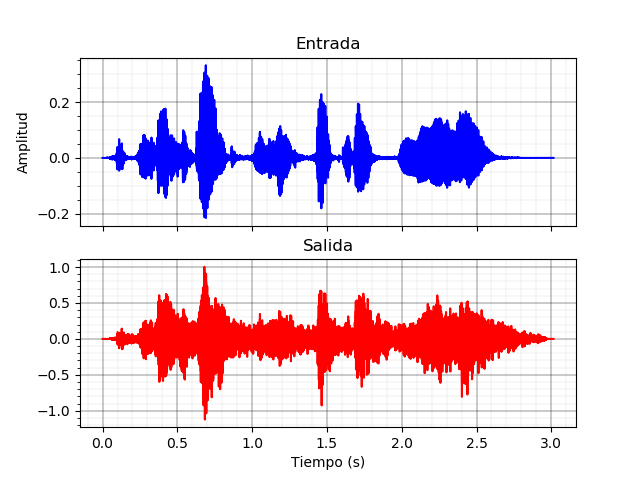
\includegraphics[scale=1]{graficos/EJ8/eco_convolucion.png}
	\caption{Resultados reverberación característica de una fábrica}
	\label{fig:bloqueElemental}
\end{figure}

Se observa como a diferencia de los casos anteriores la señal tiende mucho más a sostener sonido, esto se debe a que la respuesta al impulso es mucho más completa, y por lo tanto el sonido resultante persiste más tiempo.
El sonido que se escuchó se correspondió con un eco muy realista, que podría ser el de una fábrica


\subsection{Efectos basados en delays variables} 

Para algunos efectos, es necesario que los delays presentes en la ecuaci\'on de diferencias que describe al sistema sean variables con el tiempo. Este es el caso tanto del flanger como del vibrato.


\subsubsection{Vibrato}

El efecto de vibrato consiste en introducir peque\~nas variaciones peri\'odicas en la frecuencia, resultando en una variaci\'on peri\'odica de los tonos que se escuchan. Tomando como principio el efecto Doppler, podemos aplicar estos cambios en la frecuencia como cambios en el delay: de la misma manera que a medida que una ambulancia se aleja, se escucha m\'as grave  la sirena, si simulamos que el delay sube y baja peri\'odicamente, la nota que se escucha subir\'a y bajar\'a de la misma manera.

La ecuaci\'on que define este efecto es:
\begin{equation}
	y(n) = x\left(n - k(n) \right)
	\label{eq:vibrato}
\end{equation}

En la ecuaci\'on \ref{eq:vibrato}, $k(n)$ representa el delay variable con el tiempo, y se implementa con una senoidal que toma valores naturales entre 0 y un m\'aximo K:

\begin{equation}
	k(n) = \left \lfloor \frac{K}{2} \cdot 
		\left( 1 + \sin{\left(2\pi f_0 \cdot nT\right)} \right) \right \rfloor
		\label{eq:k(n)}
\end{equation}

Los par\'ametros que caracterizan al vibrato son pues:

\begin{equation}
	\left\{
	\begin{aligned}
		f_0	&= \text{frecuencia de modulaci\'on} \\
		K   	&= \text{profundidad de modulaci\'on}
	\end{aligned}	
	\right.
\end{equation}





\subsubsection{Flanger}

El flanger es similar al vibrato, en cuanto a que tambi\'en estar\'a presente en la salida la entrada con un delay variable. Sin embargo, la misma es sumada (con un cierto factor de ponderaci\'on) a la entrada actual, obteni\'endose:

\begin{equation}
	y(n) = x(n) + g\cdot x(n-k(n))
\end{equation}

La definici\'on de $k(n)$ que usaremos es id\'entica a la del vibrato (ecuaci\'on \ref{eq:k(n)}), es decir, una senoidal que var\'ia entre 0 y un m\'aximo.


\subsection{Robotizaci\'on}

\end{document}

